\chapter{Introduction}
\label{ch:introduction}
\section{Digital Direction Finding}

\subsection{Introduction to Digital Direction Finding}
\glspl{ddf} are an integral component of modern signal processing. They are indispensable in determining the \glspl{doa}
of incoming electromagnetic waves, thereby facilitating the localization of their sources and allowing for the
correlation of spectral components to their respective emitters.
The advancement from analog to digital systems has greatly increased the adaptability of
direction-finding technology, providing the capability for extensive monitoring over wide
frequency ranges and vast geographic areas.\\
The fields of technology leveraging digital direction finders include radar, sonar, and
radio communications. Radar systems detect and locate objects ranging from
aircraft and ships to meteorological phenomena, while sonar applications use direction
finders for underwater navigation and object detection. These technologies are indispensable
in diverse fields such as military and naval reconnaissance for localizing communication
sources and potential threats, radio astronomy for observing celestial objects emitting
radio waves, search and rescue operations to trace distress signal origins, and wireless
communications for managing and optimizing radio spectrum usage. Regardless of the application,
each relies on the accurate estimation of the \gls{doa}, underscoring the
critical and strategic importance of digital direction finders~\cite{demmel, tuncer.ch1, tuncer.ch2}.


\subsection{Types of Direction Finders}
Direction finders can be categorized into two principal classes based on their operating principles:
polarization-based and phase-based finders. Polarization-based finders utilize elementary antennas like dipole
or loop antennas, exploiting the antennas' inherent polarization characteristics to discern the direction of incoming
signals. On the other hand, phase-based finders, such as those developed by Rohde \& Schwarz, employ \glspl{uca} with
multiple aperture probes. This general approach of using an array of antennas to estimate the \gls{doa} of incoming
wavefronts is known as aperture sampling, and can be seen as a subdomain of the broader field of array processing.
These systems are capable of achieving exceptional angular resolutions across a broad frequency spectrum, ranging from
the low megahertz range to a few gigahertz~\cite{demmel}.

\autoref{fig:direction_finder_graph} provides a graph representation of commonly employed direction finding algorithms
and their inherent principles, as well as their respective strengths and weaknesses.

\begin{figure}[H]
    \centering
    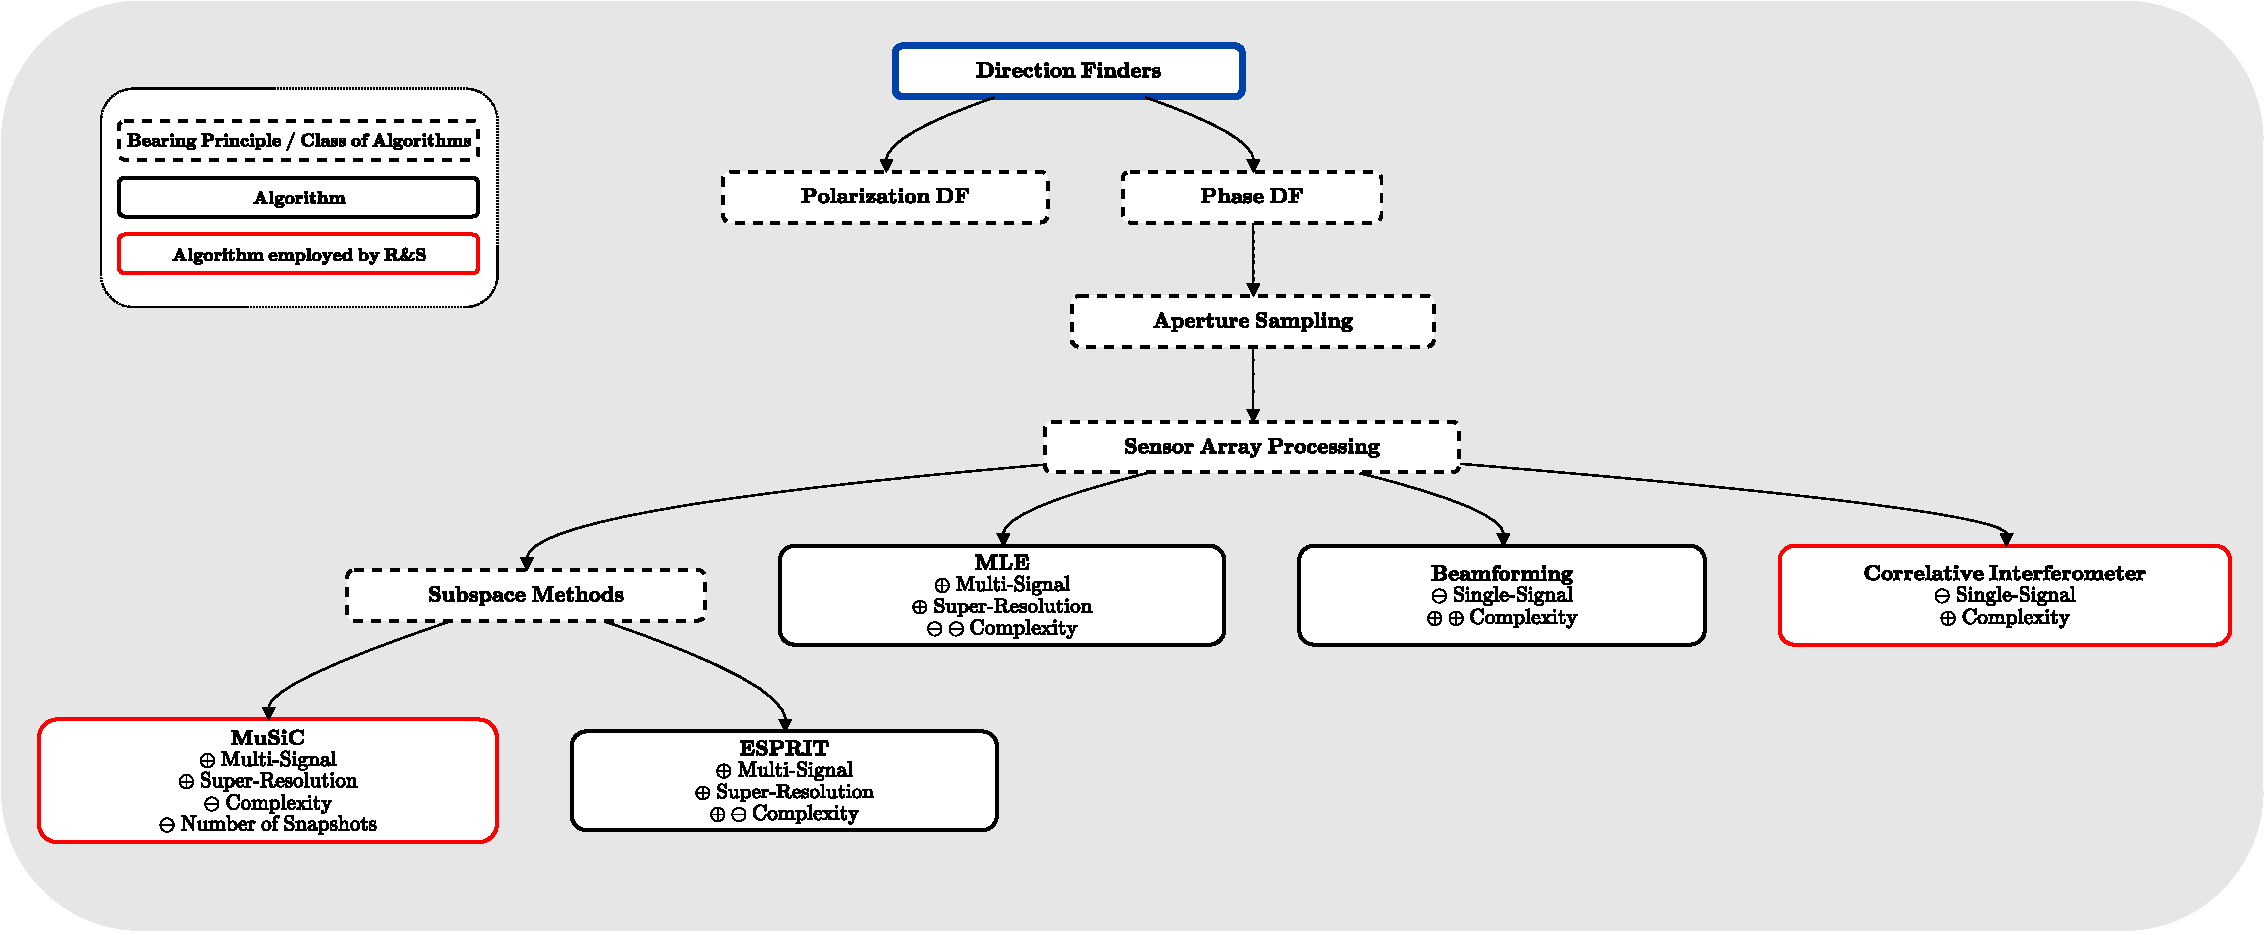
\includegraphics[width=1\textwidth]{figures/01_Introduction/direction_finder_graph.pdf}
    \caption{A graph representation of commonly employed direction finding techniques.}
    \label{fig:direction_finder_graph}
\end{figure}

\subsection{Challenges and Conventional Estimators}
In the domain of modern broadband direction finding, the accurate estimation of very short signals across extensive
bandwidths poses significant challenges. Conventional estimators, such as correlative interferometers and beamformers,
are computationally efficient and capable of providing accurate direction estimates after minimal measurements.
This efficiency renders them suitable for real-time applications and the estimation of short pulsed signals~%
\cite{meyer, tuncer.ch1, tuncer.ch2}.\\
However, these conventional methods inherently struggle with accommodating co-channel interference%
\footnote{The presence of multiple signals in the same frequency bin of the \gls{fft}.}
and multipath propagation. Additionally, they face limitations in resolving closely spaced signal sources when their
angular separation falls below the beam width of the antenna array. The performance of these methods is consequently
constrained in scenarios involving multiple incoming waves per frequency bin.\\

\subsection{Super-Resolution Methods} %TODO Subspace
To address the abovementioned limitations, super-resolution methods such as \gls{music} and \glsentryshort{esprit} are employed.
Grounded in subspace methods, these advanced techniques provide high-resolution \gls{doa} estimations and are
particularly effective in scenarios with multiple signals sharing the same frequency bin, as well as in situations where
signals have angular separations smaller than the antenna array's beamwidth. A more detailed exploration of the
\gls{music} method will be presented in \autoref{ch:OverviewMUSIC}.

Super-resolution methods are well-suited for continuous wave signals, requiring a sufficient number of
samples and a reasonable \gls{snr} to function effectively. They are capable of achieving angular resolutions as precise
as 0.1° and \glspl{rmse} of about 0.5°. However, these methods also demand higher computational resources and typically
need at least \( K \gtrsim 3M \) snapshots%
\footnote{One snapshot refers to a set of measurements that, while not necessarily captured simultaneously, are
collectively associated with a specific sampling cycle of an antenna array and includes samples from all antennas.
}
to produce reliable results, where \( M \) represents the number of antennas in
the \gls{uca}~\cite{tuncer.ch1}.


\section{Model Order Estimation}
The effectiveness of the aforementioned super-resolution methods relies on accurate estimates of the model order,
denoted as \( N \). This model order reflects the number of co-channel wavefronts concurrently impinging on the sensor array.\\
\gls{moe} is fundamentally grounded in the analysis of the eigenvalue profile of the signal's covariance matrix.
This analysis aims to distinguish signal eigenvalues from a cluster of low variance noise eigenvalues.
In an ideal scenario, the set of noise eigenvalues would have zero variance, facilitating a distinct separation between
signal and noise subspaces.\\
The classical \glspl{ic}, such as \gls{aic} and \gls{mdl}, which have been foundational in the field
for decades, will be elaborated in \autoref{sec:ClassicalInformationCriteria}.\\
The comprehensive discussion on the theoretical methodologies, including covariance matrix analysis, subspace concepts,
and the mathematical models underlying \gls{moe} and \gls{doa} estimation, will be detailed in \autoref{chap:DataModel}.


\subsection{Challenges in Conventional MOE}
While conventional \gls{moe} techniques, such as the \glspl{ic} \gls{aic} and \gls{mdl}, offer closed-form
solutions~\cite{barthelme2020}, making them relatively computationally efficient, they often falter under non-ideal
conditions:

\begin{itemize}
    \item \textbf{Low SNR:} In scenarios with low \glspl{snr}, these methods tend to underfit the model
    order, resulting in unreliable estimates~\cite{eft, yu22RCNN}.
    \item \textbf{High SIR:} With high \glspl{sir}, estimation errors increase without showing a distinct bias
    towards either overfitting or underfitting.
    \item \textbf{Sub-Sampled Covariance Matrix:} Utilizing sub-sampled covariance matrices decreases the goodness of fit
    of the estimated covariance matrix, leading to an increased variance in noise eigenvalues, a departure from theoretically
    expected noise eigenvalue distributions~\cite{meyer}, and the occurrence of negative eigenvalues~\cite{barthelme21sub, meyer}.
    \item \textbf{Limited Snapshots:} A limited number of signal snapshots%
\footnote{This tends to be the case when the number of snapshots \( K \) is of the same order as the number of antennas \( M \)~\cite{eft}}.
    affects the fidelity of the eigenvalue estimates~\cite{eft, barthelme2020, barthelme21sub}.
    \item \textbf{Coherent Multipath Interference:} Such interference typically results in overfitting, with the methods
    incorrectly interpreting multipath signals as separate, independent sources~\cite{yu22RCNN}.
    \item \textbf{Non-Gaussian Noise:} These estimators are designed to assume \gls{awgn}. Therefore, their performance
    is negatively impacted in the presence of non-Gaussian noise, especially in higher frequency ranges.
    \item \textbf{Susceptibility to Overfitting:} \gls{aic} and \gls{mdl} have been found to be generally prone to
    overfitting, especially when dealing with lower model orders~\cite{barthelme2020, eft}.
\end{itemize}

\subsection{Advancements in MOE}

\subsubsection*{Exponential Fitting Test (EFT)}
The \gls{eft} marks an algorithmic advancement in \gls{moe} for incoherent scenarios with a low number of snapshots and
the presence of non-Gaussian noise.
Introduced in~\cite{eft}, the \gls{eft} leverages the observation that noise eigenvalues approximately exhibit exponential
decay. It aims to detect mismatches greater than a threshold value between observed eigenvalues and the assumed exponential
profile, thereby effectively discerning signal from noise.
Despite subsequent enhancements to the \gls{eft} as detailed in~\cite{costa2007} and~\cite{costa2009}, the original

version still provides a baseline for comparative analysis against classical methods like \gls{aic} and \gls{mdl} and
the \glspl{dnn} explored in this thesis. A detailed elaboration on the \gls{eft} algorithm will be presented in \autoref{sec:eft}.

\subsubsection*{Recent Deep Learning Approaches}
The latest advancements in \gls{moe} have demonstrated the superiority of data-driven approaches, through the employment
of \glspl{dnn} over classical methods.
Research highlighted in~\cite{barthelme2020, barthelme21sub, yu22RCNN, yang2020, rogers2021} shows that \glspl{dnn}
outperform classical methods in terms of accuracy and computational efficiency, particularly in
challenging scenarios with sub-array sampling, multipath interference, and low numbers of snapshots.\\
These advanced \glspl{dnn} approaches represent a significant shift in \gls{moe}, providing more robust and adaptable
solutions in complex signal environments. A concise exploration of these DL-driven advancements in \gls{moe} will be
detailed in \autoref{sec:dl-advancements} before we will present our own \gls{dnn} approaches in \autoref{ch:model_exploration}
the choice for the input data and the underlying datasets in \autoref{ch:dataset_generation}.
The final chapters will than elaborate on the results and will also demonstrate the before mentioned caveats of the
classical approaches and we will end with a conclusion and outlook upon suggested future work in the field of \gls{moe}
in \autoref{ch:outlook}.

\endinput

% Recent advancements have demonstrated the superiority of data-driven approaches, particularly in the realm of
% \glspl{dnn}, for \gls{moe} \cite{barthelme2020, barthelme21sub, yu22RCNN, yang2020, rogers2021}. These DNN-based models have been shown to excel in MOE tasks,
% surpassing classical methods in accuracy and computational efficiency, especially in challenging scenarios with sub-array
% sampling. The study \cite{barthelme21sub} specifically highlights the effectiveness of NN-based estimation schemes in
% outperforming traditional estimators in both estimation accuracy and computational complexity.
% These innovative approaches represent a paradigm shift in MOE, offering more robust and adaptable solutions in complex
% signal environments.

% While many means towards improving the performance of these classical methods have been proposed, the latest research
% has shown the <überlegenheit> of fully data-driven approaches in the domain of \glspl{dnn}~\cite{barthelme2020, yu22RCNN}.
% - briefly mention the adaptations of classical methods:
% These limitations underscore the need for more robust and adaptable MOE methods, particularly in complex signal environments where traditional criteria may not provide accurate estimations.



% ---

% \cite{barthelme21sub}
% is the only paper that discusses DL-driven sulutions for \gls{doa} estimation and \gls{moe} in context of sub-array sampling.
% simulations show that the proposed NN-based estimation scheme iable to outperform the state-of-the-art estimators in terms of estimation accuracy and computational complexity

% \endinput